

\section{Visão Geral do Conjunto de Dados}
% estatisticas calculadas lá no notebook



\section{Preparação do Conjunto de Dados}

\begin{table}[h!]
	\centering
	\caption{Divisão dos dados}
	\label{tab:divisao-dados}
	%\scalefont{0.77}
	\begin{tabular}{c c c c c}
		\toprule
		\textbf{Abordagem} & \textbf{Tipo de Exemplo} & \textbf{Treino} & \textbf{Validação} & \textbf{Teste}\\
		\midrule
		\multirow{2}{*}{1} & genuíno & 2011 & 299 & 618 \\
     & forjado & 11649 & 1648 & 3237 \\
     \midrule
    \multirow{2}{*}{2} & genuíno & 2011 & 299 & 618   \\
     & forjado & 2024 & 308 & 569 \\
		\bottomrule
	\end{tabular}
\end{table}

\begin{figure}[h!]
  \centering
\caption{Visualização da divisão dos dados}
  \subfloat[Abordagem 1\label{subfig:approach1}]{%
    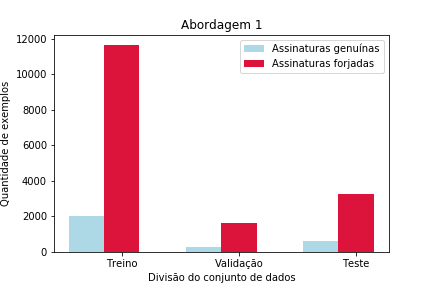
\includegraphics[width=0.7\textwidth]{imgs/approach1}
  }
  \hfill
  \subfloat[Abordagem 2\label{subfig:approach2}]{%
    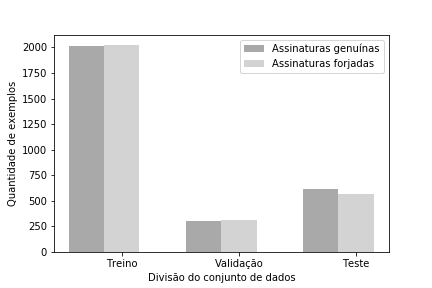
\includegraphics[width=0.7\textwidth]{imgs/approach2}
  }
  \label{fig:divisao-dados}
\end{figure}
